% --------------------------------------------------------------
% This is all preamble stuff that you don't have to worry about.
% Head down to where it says "Start here"
% --------------------------------------------------------------
 
\documentclass[12pt]{article}
\usepackage[utf8]{inputenc} 
\usepackage[ngerman]{babel} 
\usepackage[T1]{fontenc} 
\usepackage[a4paper,left=20mm,right=20mm,top=10mm,bottom=10mm,headheight=12pt, headsep=0pt, nohead, nofoot]{geometry}
\usepackage{amsmath,amsthm,amssymb}
\usepackage{graphicx}
 
\newcommand{\N}{\mathbb{N}}
\newcommand{\Z}{\mathbb{Z}}
 
\newenvironment{theorem}[2][Theorem]{\begin{trivlist}
\item[\hskip \labelsep {\bfseries #1}\hskip \labelsep {\bfseries #2.}]}{\end{trivlist}}
\newenvironment{lemma}[2][Lemma]{\begin{trivlist}
\item[\hskip \labelsep {\bfseries #1}\hskip \labelsep {\bfseries #2.}]}{\end{trivlist}}
\newenvironment{exercise}[2][Exercise]{\begin{trivlist}
\item[\hskip \labelsep {\bfseries #1}\hskip \labelsep {\bfseries #2.}]}{\end{trivlist}}
\newenvironment{reflection}[2][Reflection]{\begin{trivlist}
\item[\hskip \labelsep {\bfseries #1}\hskip \labelsep {\bfseries #2.}]}{\end{trivlist}}
\newenvironment{proposition}[2][Proposition]{\begin{trivlist}
\item[\hskip \labelsep {\bfseries #1}\hskip \labelsep {\bfseries #2.}]}{\end{trivlist}}
\newenvironment{corollary}[2][Corollary]{\begin{trivlist}
\item[\hskip \labelsep {\bfseries #1}\hskip \labelsep {\bfseries #2.}]}{\end{trivlist}}
 
\begin{document}
 
% --------------------------------------------------------------
%                         Start here
% --------------------------------------------------------------
 
\title{COBRA industrial robot Kinematic}%replace X with the appropriate number
\author{Sandra Schuhmacher \& Daniel Veeckman} %if necessary, replace with your course title
 
\maketitle

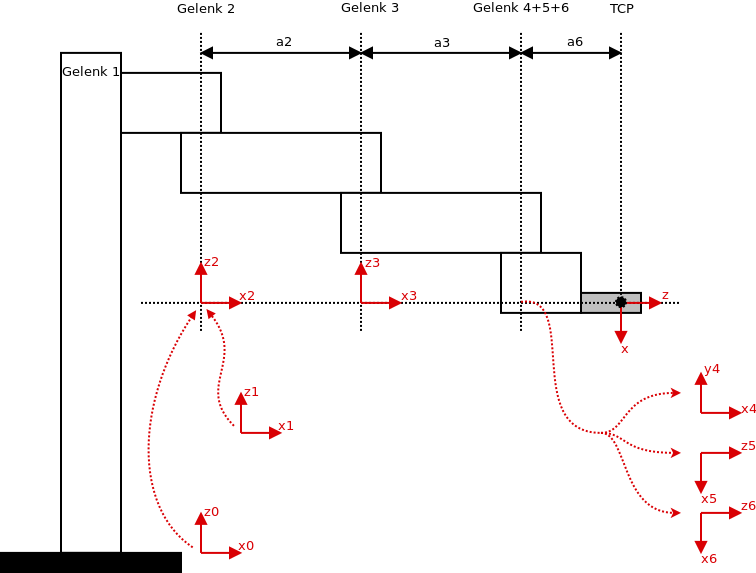
\includegraphics[width=0.6\textwidth]{Kinematic.png}
 
\section{Gelenke}

\begin{align*}
    d_1 &= d_1 & q_1 &= 0^\circ \\
    d_2 &= 0   & q_2 &= \theta_2 \\
    d_3 &= 0   & q_3 &= \theta_3 \\
    d_4 &= 0   & q_4 &= \theta_4 \\
    d_5 &= 0   & q_5 &= \theta_5 \\
    d_6 &= 0   & q_6 &= \theta_6 \\
\end{align*}
 
\section{Armteile}

\begin{align*}
    a_1 &= a_1 & \alpha_1 &= 0^\circ \\
    a_2 &= 0   & \alpha_2 &= 0^\circ \\
    a_3 &= 0   & \alpha_3 &= 0^\circ \\
    a_4 &= 0   & \alpha_4 &= 90^\circ \\
    a_5 &= 0   & \alpha_5 &= 90^\circ \\
    a_6 &= 0   & \alpha_6 &= 0^\circ \\
\end{align*}
 
\end{document}